\PassOptionsToPackage{dvipsnames,table}{xcolor}
\documentclass[10pt]{beamer}
\usepackage{Cours}

\begin{document}

\input{\detokenize{/home/fenarius/Travail/Cours/NSITerminale/docs/commun/MacrosCours.tex}}
\setcounter{numchap}{0}
\newcommand{\Systeme}{\cnum Révisions : ligne de commande}
\newcommand{\Turtle}{\cnum Aide mémoire de turtle}
\newcommand{\Python}{\cnum Révisions : base de Python}

\pythonmode


% Manipulation des dossiers
\begin{frame}
	\mframe{\Systeme}
	\begin{block}{Ligne de commande : manipulation des dossiers}
		\begin{description}
			\item<1->[\pmc{pwd}] permet d'afficher le chemin complet du dossier dans lequel on se trouve.
			\item<2->[\pmc{cd}] permet de changer le dossier courant, on indique le dossier de destination :
			      \onslide<3->{\begin{itemize}
					      \item de façon absolue, c'est à dire depuis la racine du système de fichier
					      \item de façon relative, c'est à dire depuis le dossier courant, dans ce cas \og \texttt{..} \fg indique le dossier parent.
				      \end{itemize}}
			\item<4->[\pmc{mkdir}] permet de créer un dossier
			\item<5->[\pmc{rmdir}] permet d'effacer un dossier vide
			\item<6->[\pmc{mv}] permet de renommer ou de déplacer un dossier (fonctionne aussi sur les fichiers)
		\end{description}
	\end{block}
\end{frame}

\begin{frame}
	\mframe{\Systeme}
	\begin{block}{Ligne de commande : manipulation des fichiers}
		\begin{description}
			\item<2->[\pmc{ls}] permet de lister le contenu d'un dossier, parmi les options les plus courantes on trouve :
			      \onslide<3->{\begin{itemize}
					      \item[\pmc{ls -l}] pour voir les droits sur les  fichiers
					      \item[\pmc{ls -a}] pour voir les  fichiers cachés, c'est à dire ceux dont le nom commence par un point \texttt{.}
				      \end{itemize}}
			\item<4->[\pmc{cat}] permet de visualiser le contenu d'un fichier texte
			\item<5->[\pmc{touch}] permet de créer un fichier vide
			\item<6->[\pmc{rm}] permet d'effacer un fichier
			\item<6->[\pmc{cp}] permet de copier un fichier
		\end{description}
	\end{block}
\end{frame}


\begin{frame}
	\mframe{\Systeme}
	\begin{block}{Ligne de commande : gestion des permissions}
		\onslide<2->{Trois type de droits sont définis :}
		\begin{description}
			\item<3->[\pmc{r}] droit de lecture du fichier
			\item<4->[\pmc{w}] droit d'écriture  dans le fichier
			\item<5->[\pmc{x}] droit d'execution du fichier
		\end{description}
		\onslide<6->{Ces droits sont définis pour : }
		\begin{description}
			\item<7->[\pmc{u}] le propriétaire du fichier
			\item<8->[\pmc{g}] le groupe  du fichier
			\item<9->[\pmc{o}] tous les autres utilisateurs
		\end{description}
	\end{block}
\end{frame}

\begin{frame}
	\mframe{\Systeme}
	\begin{block}{Ligne de commande : commande \textcolor{yellow}{\tt chmod}}
		\begin{itemize}
			\item<2-> L'affichage des droits sur un fichier se fait en affichant un tiret \texttt{-} si le droit est absent ou la lettre (\texttt{r}, \texttt{w}, \texttt{x}) désignant le droit sinon. On liste dans l'ordre les droits du propriétaire, puis ceux groupe puis ceux des autres. Par exemple :  \\
			      \begin{itemize}
				      \item<3-> {{\texttt{rw-r-----} :}} \onslide<4-> {L'utilisateur a les droits d'écriture et de lecture, le groupe a le droit de lecture, les autres n'ont aucun droit}
				      \item<5-> {{\texttt{rwxr-xr-x} :}} \onslide<6-> {L'utilisateur a les droits d'écriture, de lecture et d'exécution, le groupe et les autres ont le droit de lecture et d'exécution}
			      \end{itemize}
			\item<7-> La commande \pmc{chmod} permet de modifier les droits sur un fichier dont on est propriétaire. En voici quelques exemples :
			      \begin{itemize}
				      \item<8->{\pmc{chmod} {\tt g+w monfichier} :} \onslide<9->{Ajoute (\texttt{+}) au groupe (\texttt{g}) le droit d'écriture (\texttt{w})}
				      \item<10->{\pmc{chmod} {\tt u+x monfichier} :} \onslide<11->{Ajoute (\texttt{+}) au propriétaire (\texttt{u}) le droit d'éxécution (\texttt{x})}
				      \item<12->{\pmc{chmod} {\tt  og-r monfichier} :} \onslide<13->{Enlève (\texttt{-}) au groupe et aux autres (\texttt{og}) le droit de lecture (\texttt{r})}
				      \item<13->{\pmc{chmod} {\tt a-r monfichier} :} \onslide<13->{Enlève (\texttt{-}) à tout le monde (\texttt{a}) le droit de lecture (\texttt{r})}
			      \end{itemize}
		\end{itemize}
	\end{block}
\end{frame}


% Turtle : papier et crayon
\begin{frame}[fragile]
	\mframe{\Turtle}
	\begin{block}{Création du papier et du crayon}
		\begin{lstlisting}
	import turtle
	papier = turtle.Screen()
	crayon = turtle.Turtle()
		\end{lstlisting}
	\end{block}
	\onslide<2->{\begin{block}{Remarques}
			On peut créer simultanément plusieurs crayons, l'instruction \pmc{reset} permet d'effacer la totalité des tracés d'un crayon.
		\end{block}}
\end{frame}

% Turtle : papier et crayon 1/2
\begin{frame}[fragile]
	\mframe{\Turtle}
	\begin{block}{Propriétés du crayon}
		\begin{itemize}
			\item<2-> \pmc{pensize} pour l'épaisseur du trait.
			\item<3-> \pmc{color} pour changer la couleur.
			\item<4-> \pmc{penup} et \pmc{pendown} pour relever ou abaisser le crayon.
			\item<5-> \pmc{hideturtle} et \pmc{showturtle} pour masquer ou faire apparaître le crayon.
			\item<6-> \pmc{speed} pour modifier la vitesse de tracé.
		\end{itemize}
	\end{block}
\end{frame}

% Turtle : papier et crayon 2/2
\begin{frame}[fragile]
	\mframe{\Turtle}
	\begin{block}{Propriétés du crayon}
		\begin{itemize}
			\item \pmc{pensize} pour l'épaisseur du trait.
			\item \pmc{color} pour changer la couleur.
			\item \pmc{penup} et \pmc{pendown} pour relever ou abaisser le crayon.
			\item \pmc{hideturtle} et \pmc{showturtle} pour masquer ou faire apparaître le crayon.
			\item \pmc{speed} pour modifier la vitesse de tracé.
		\end{itemize}
	\end{block}
	\begin{exampleblock}{Exemple}
		\begin{lstlisting}
	# Crayon abaissé, rouge, d'épaisseur 3, caché et se déplaçant à la vitesse maximum
	crayon.pendown()
	crayon.pensize(3)
	crayon.color("red")
	crayon.hideturtle()
	crayon.speed(10)
		\end{lstlisting}
	\end{exampleblock}
\end{frame}

% Turtle : Orientation et déplacement
\begin{frame}[fragile]
	\mframe{\Turtle}
	\begin{block}{Orientation du crayon}
		\begin{itemize}
			\item<2-> \pmc{setheading} pour fixer l'orientation de la tortue à un angle donnée.
			\item<3-> \pmc{left} pour tourner vers la gauche du nombre de degrés donné.
			\item<4-> \pmc{right} pour tourner vers la droite du nombre de degrés donné.
		\end{itemize}
	\end{block}
	\onslide<5->{\begin{block}{Déplacement du crayon}
			\begin{itemize}
				\item<5-> \pmc{goto} pour envoyer la tortue au point de coordonnées {\tt (x,y)}.
				\item<6-> \pmc{forward} pour faire avancer la tortue de la distance indiquée.
				\item<7-> \pmc{backward} pour faire reculer la tortue de la distance indiquée.
			\end{itemize}
		\end{block}}
\end{frame}

% Turtle : Tracé d'un carré
\begin{frame}[fragile]
	\mframe{\Turtle}
	\begin{exampleblock}{Tracé d'un carré}
		\begin{lstlisting}
	crayon.penup()
	crayon.setheading(0)
	crayon.goto(-100,-100)
	for _ in range(4):
		crayon.forward(100)
		crayon.left(90)
		\end{lstlisting}
		\onslide<2->{\begin{center}
			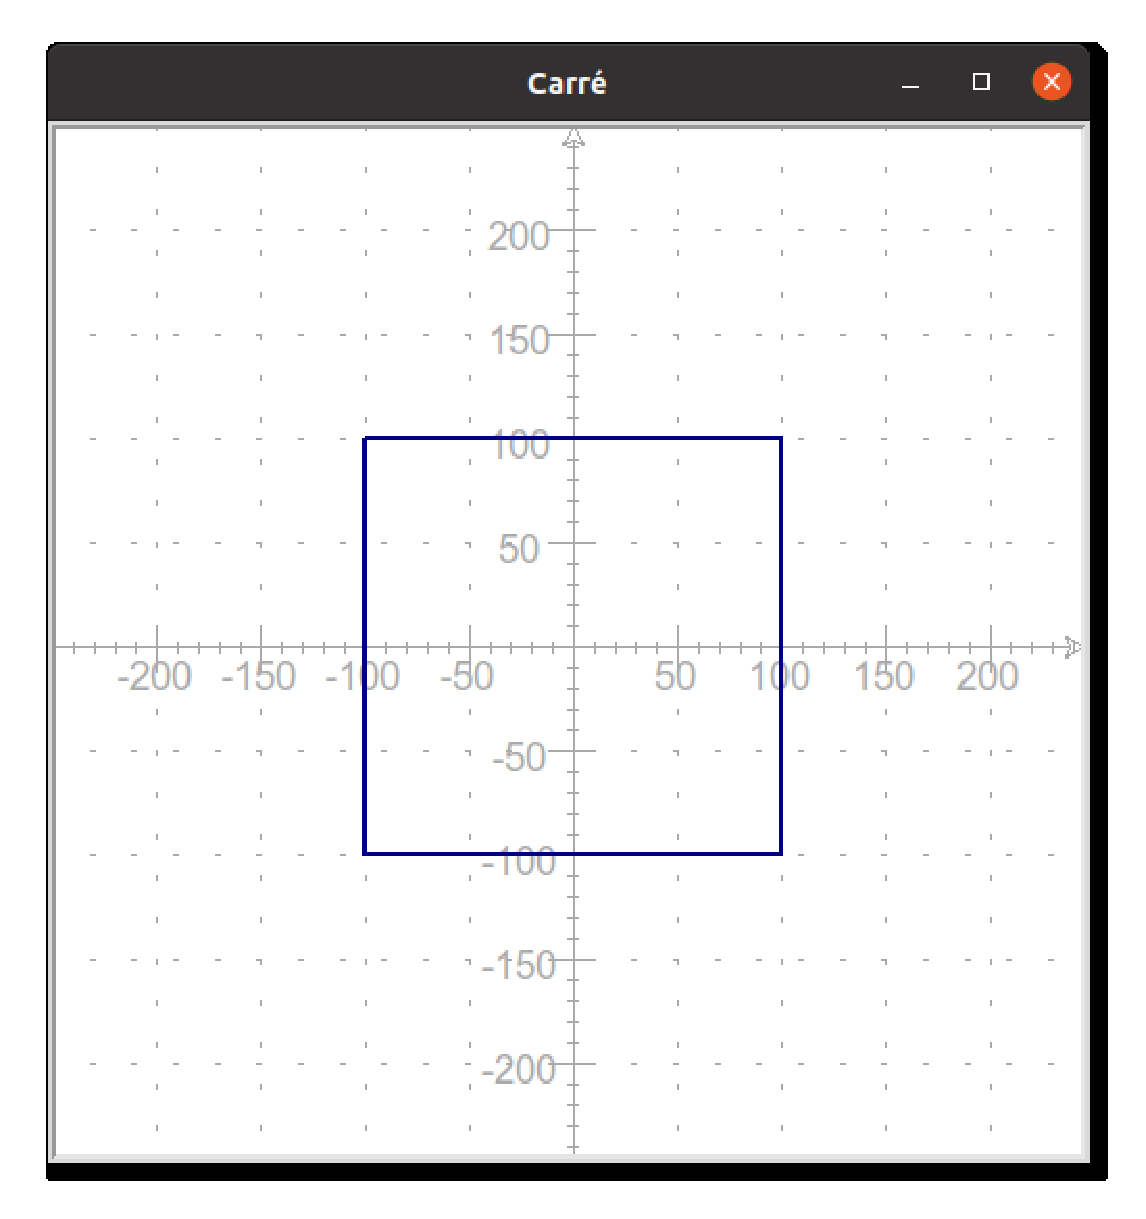
\includegraphics[width=100px]{carre.eps}}
		\end{center}
	\end{exampleblock}
\end{frame}


% Python
\begin{frame}[fragile]
	\mframe{\Python}
	\begin{block}{Programmation en python : généralités}
		\begin{itemize}
			\item<1-> Python renvoie un message d'erreur lorsqu'il n'arrive pas à interpréter les instructions de votre programme. Prendre l'habitude de \textcolor{blue}{lire attentivement} ces messages, qui sont de premiers indices pour déterminer la source de l'erreur
			\item<2-> En Python, les \textcolor{blue}{commentaires} s'écrivent en faisant commencer la ligne par le caractère \textcolor{red}{\tt \#}.
			\item<3-> Le respect de la syntaxe du langage est fondamentale et demande de la rigueur, prendre garde notamment au respect de l'\textcolor{blue}{indentation}.
			\item<4-> Attention aussi à bien surveiller les correspondances entre les parenthèses mais aussi les guillemets ou les apostrophes qui sont souvent source d'erreurs.
		\end{itemize}
	\end{block}
\end{frame}



% Instructions conditionnelles
\begin{frame}[fragile]
	\mframe{\Python}
	\begin{alertblock}{Instructions conditionnelles}
		\begin{itemize}
			\item<2-> La syntaxe d'une instruction conditionnelle en Python est :
			      \begin{lstlisting}
	if <condition>:
		<instructions1>
	else:
		<instructions2>
	\end{lstlisting}
			      Cela permet d'exécuter les {\tt <instructions1>} si la {\tt condition} est vérifiée, sinon on exécute les {\tt <instructions2>}.
			\item<3->  \textcolor{red}{\danger} On fera bien attention à la syntaxe du langage, et notamment à l'usage du caractère \textcolor{red}{\tt :} qui suit la condition (et le {\tt else}) et à l'\textcolor{red}{indentation}, c'est à dire le décalage des instructions qui doivent s'executer.
		\end{itemize}
	\end{alertblock}
\end{frame}

% Exemple instructions conditionnelles
\begin{frame}[fragile]
	\mframe{\Python}
	\begin{exampleblock}{Exemple de {\tt if \dots else}}
		Compléter le programme suivant afin qu'il affiche  "positif" si la variable \texttt{r} est supérieur à 0 et "négatif" sinon
		\begin{lstlisting}
	..... r>=0 ..
		.....("positif")
	....:
		..........
	\end{lstlisting}
	\end{exampleblock}
\end{frame}

\begin{frame}[fragile]
	\mframe{\Python}
	\begin{exampleblock}{Exemple de {\tt if \dots else}}
		Compléter le programme suivant afin qu'il affiche  "positif" si la variable \texttt{r} est supérieur  ou égale à 0 et "négatif" sinon
		\begin{lstlisting}
	if r>=0:
		print("positif")
	else:
		print("négatif")
	\end{lstlisting}
	\end{exampleblock}
\end{frame}




% boucle for
\begin{frame}[fragile]
	\mframe{\Python}
	\begin{alertblock}{Boucles {\tt for}}
		\begin{itemize}
			\item<2-> Les instructions :
			      \begin{lstlisting}
	for <variable> in range(<entier>):
		 <instructions>
	\end{lstlisting}
			      permet de créer une variable parcourant les entiers de 0 à {\tt <entier>} (exclu).
			\item<3-> Les {\tt <instructions>} indentées qui suivent seront executées pour chaque valeur prise par la variable.
			\item<4-> La boucle {\tt for} permet donc de répéter un nombre prédéfini de fois des instructions, on dit que c'est une boucle bornée.
		\end{itemize}
	\end{alertblock}
\end{frame}



% Exemple for
\begin{frame}[fragile]
	\mframe{\Python}
	\begin{exampleblock}{Exemple de {\tt for \dots range}}
		Quel sera l'affichage produit par le programme suivant ? Expliquer
		\begin{lstlisting}
	for cpt in range(0,5):
		print(cpt)
	\end{lstlisting}
		\onslide<2-> \textcolor{OliveGreen}{Ce programme affiche "0 1 2 3 4". En effet, la variable {\tt cpt} parcourt les valeurs entières de 0 à 5 mais 5 est exclu. Et à chaque tour de boucle on affiche cette variable grâce à un {\tt print}.}
	\end{exampleblock}
\end{frame}


% Appel à une fonction
\begin{frame}[fragile]
	\mframe{\Python}
	\begin{alertblock}{Définir une fonction en Python}
		Pour définir une fonction en Python, on utilise la syntaxe suivante :
		\begin{lstlisting}
	def <nom_fonction>(<arguments>):
		<instruction>
		return <resultat>
	\end{lstlisting}
	\end{alertblock}
\end{frame}


% Appel à une fonction
\begin{frame}[fragile]
	\mframe{\Python}
	\begin{alertblock}{Définir une fonction en Python}
		Pour définir une fonction en Python, on utilise la syntaxe suivante :
		\begin{lstlisting}
	def <nom_fonction>(<arguments>):
		<instruction>
		return <resultat>
	\end{lstlisting}
	\end{alertblock}
	\begin{exampleblock}{Exemple}
		\begin{lstlisting}
	def plus_grand(a,b):
		if a>b:
			pg=a
		else:
			pg=b
		return pg
	\end{lstlisting}
	\end{exampleblock}
\end{frame}

% Exemples
\begin{frame}[fragile]
	\mframe{\Python}
	\begin{exampleblock}{Exercices}
		\begin{enumerate}
			\item On considère la fonction définie ci-dessous :
			      \begin{lstlisting}
		def calcul(x,y):
			res = 10*x+y
			return res
				\end{lstlisting}
			      Quel sera la valeur de {\tt calcul(2,5)} ? \\
				  \onslide<2->\textcolor{OliveGreen}{\tt calcul(2,5)=25}
			\item Ecrire une fonction {\tt est\_pair(n)} qui renvoie {\tt True} lorsque l'entier {\tt n} est pair et {\tt False} sinon.
		\end{enumerate}
	\end{exampleblock}
\end{frame}

\begin{frame}[fragile]
	\mframe{\Python}
	\begin{exampleblock}{Correction}
			      \begin{lstlisting}
		def est_pair(n):
		''' Renvoie True ou False suivant que n est pair ou non'''
		assert type(n)==int, "le paramètre n'est pas un nombre entier"
		if n%2==0:
			return True
		else:
			return False
				\end{lstlisting}
	On peut remarquer que c'est la valeur du booléen {\tt n\%2==0} qui est renvoyé et donc simplifier l'écriture de cette fonction :
	\end{exampleblock}
\end{frame}


\begin{frame}[fragile]
	\mframe{\Python}
	\begin{exampleblock}{Correction (meilleure version)}
			      \begin{lstlisting}
		def est_pair(n):
		''' Renvoie True ou False suivant que n est pair ou non'''
		assert type(n)==int, "le paramètre n'est pas un nombre entier"
		return n%2==0
				\end{lstlisting}
	\end{exampleblock}
\end{frame}


% Représentation listes
\begin{frame}
	\mframe{\Python}
	\begin{alertblock}{Indice d'un élément}
		\begin{itemize}
			\item<1-> Les éléments d'une liste sont repérés par leur position dans la liste, on dit leur \textcolor{blue}{indice} \\
			\item<2-> Attention, la numérotation commence à zéro, l'indice du premier élément de la liste est donc zéro
			\item<3-> On peut accéder à un élément en indiquant le nom de la liste puis  l'indice de cet élément entre crochet
			\item<4-> L'erreur {\tt IndexError} indique qu'on tente d'accéder à un indice qui n'existe pas.
		\end{itemize}
		\onslide<4->{\begin{center}
				Une liste L : \\
				\begin{tabularx}{0.8\textwidth}{l|Y|Y|Y|Y|Y|}
					\cline{2-6}
					Eléments                    & {\tt L[0]}                       & {\tt L[1]}                       & {\tt L[2]}                       & {\tt L[3]}                       & {\tt L[4]}                       \\
					\cline{2-6}
					\multicolumn{1}{c}{ }       & \multicolumn{1}{c}{$\downarrow$} & \multicolumn{1}{c}{$\downarrow$} & \multicolumn{1}{c}{$\downarrow$} & \multicolumn{1}{c}{$\downarrow$} & \multicolumn{1}{c}{$\downarrow$} \\
					\multicolumn{1}{c}{Indices} & \multicolumn{1}{c}{0}            & \multicolumn{1}{c}{1}            & \multicolumn{1}{c}{2}            & \multicolumn{1}{c}{3}            & \multicolumn{1}{c}{4}            \\
				\end{tabularx}
			\end{center}}
	\end{alertblock}
\end{frame}


% Manipulation des listes
\begin{frame}
	\mframe{\Python}
	\begin{alertblock}{Opérations sur les listes}
		Les opérations suivantes permettent de manipuler les listes (ajout, suppression, insertion d'éléments). On fera bien attention à la syntaxe on met le nom de la liste suivi d'un point suivi de l'opération à effectuer (voir exemples)
		\begin{itemize}
			\item<1-> \textcolor{blue}{\tt remove} permet de supprimer un élément d'une liste. Par exemple : {\tt ma\_liste.remove(elt)} va enlever {\tt elt} de {\tt ma\_liste}.
			\item<2-> \textcolor{blue}{\tt append} permet d'ajouter un élément à la fin d'une liste. Par exemple : {\tt ma\_liste.append(elt)} va ajouter {\tt elt} à la fin de {\tt ma\_liste}.
			\item<3-> \textcolor{blue}{\tt insert} permet d'insérer un élément à un indice donnée. Par exemple : {\tt ma\_liste.insert(indice,elt)} va insérer {\tt elt} dans {\tt ma\_liste} à l'index {\tt indice}.
			\item<4-> \textcolor{blue}{\tt pop} permet de récupérer un élement de la liste tout en le supprimant de la liste. Par exemple {\tt elt=ma\_liste.pop(2)} va mettre dans {\tt elt} {\tt ma\_liste[2]} et dans le même temps supprimer cet élément de la liste.
		\end{itemize}
	\end{alertblock}
\end{frame}


% Génération de listes
\begin{frame}
	\mframe{\Python}
	\begin{alertblock}{Création de listes}
		On peut créer des listes de diverses façons en Python :
		\begin{itemize}
			\item<2-> \textcolor{red}{Par ajout succesif d'élement} on part alors d'une liste (éventuellement vide) et on ajoute chaque élément à l'aide d'instruction \textcolor{blue}{\tt append}.
			\item<3-> \textcolor{red}{Par répétition du même élément} on utilise alors le caractère \textcolor{blue}{\tt *} pour indiquer le nombre de répétitions. \\
			      \onslide<4-> {Par exemple pour créer la liste: \\ {\tt bavardages = ["bla", "bla", "bla", "bla"]} \\ on peut simplement écrire : \\}
			      \onslide<5->{\textcolor{blue}{\tt bavardages = ["bla"]*4}}
			\item<6->	 \textcolor{red}{Par compréhension}, c'est à dire en indiquant la définition des éléments qui composent la liste. \\
			      \onslide<7-> {Par exemple la liste {\tt puissances2 = [1, 2, 4, 8, 16, 32, 64, 128]} est constitué des huits premières puissances de 2} \\
			      \onslide<8-> {Elle contient donc $2^0, 2^1, 2^2, \dots 2^7$, ce qui se traduit en Python par :}\\
			      \onslide<9-> \textcolor{blue}{\tt puissances2 = [2**k for k in range(8)]}
		\end{itemize}
	\end{alertblock}
\end{frame}
\end{document}
